\begin{center}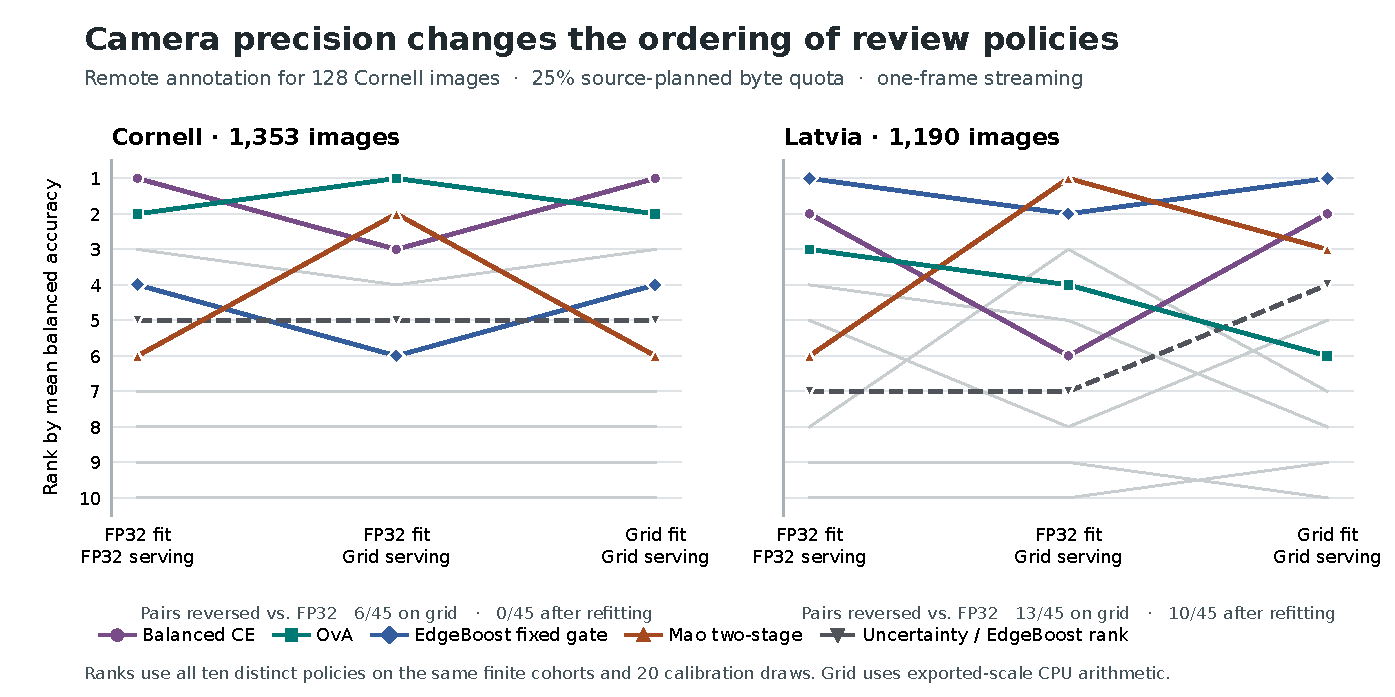
\includegraphics[width=.96\linewidth]{figures/precision_ranks.pdf}\end{center}
\note{Figure 3. Precision effects under the former Cornell-trained protocol. Identical calibration draws, test images and quotas isolate changes in numerical representation. The grid is evaluated on the host.}

\sect{5 \quad Where the Latvian errors move}
We first separate operating point from score ordering, using the nine later capture days and exactly the same photographs for each model. This exploratory analysis followed the acquisition comparison. Cutoffs maximize balanced accuracy on 32 early paid labels, with no late label used. Refitting the head uses the same labels. No cloud decisions enter this diagnostic.
\begin{center}\small
\begin{tabular}{@{}lrrrr@{}}\toprule
Pipeline & Source AUC & Cutoff-only BA & Refit AUC & Refit BA\\\midrule
V2 &0.449&48.17&0.477&48.67\\
V2-grid &0.408&46.06&0.510&50.97\\
V4 &0.791&65.88&0.622&55.92\\\bottomrule
\end{tabular}
\end{center}
For V2 the source ranking is weak even before threshold selection. Optimizing its cutoff on the test references as a diagnostic upper bound gives only 51.57\% BA. This same bound reaches 74.07\% for V4. Across the matched images the two baselines already make different errors. V2 has 67 false alarms and 49 misses, while V4 has 12 false alarms and 227 misses. The observed shift concerns the source training task, feature ordering and operating point. Latvia's negative label means no visible scab and can include other damage. The data cannot separate that difference from acquisition conditions or lesion severity.

\newpage
\subt{A protected alert is a stronger zero-label control}
For the protection variant, every original disease alert stays positive. Queries consider only the other photos. This guarantees no extra misses relative to the original camera on a fixed sequence and gives no guarantee about false alarms. At zero initial credit and a 32-label allowance, the following rows include the same spending ceiling.
\begin{center}\small
\begin{tabular}{@{}lrrr@{}}\toprule
Mean false alarms / misses & V2 & V2-grid & V4\\\midrule
Native score, no review &67/49&67/68&12/227\\
Frozen with protection and review &67/31&67/45&12/206\\
Adaptive purchase with protection &67/32&67/47&15.05/196.05\\\bottomrule
\end{tabular}
\end{center}
The V4 purchase with protection removes 9.95 additional misses but adds 3.05 false alarms relative to the protected zero-label comparison. Holding its number of net alerts fixed by random reassignment within the corresponding source prediction groups explains 9.57 of those recovered positives. The more targeted component accounts for 0.38 per draw in that comparison. Nine leave-one-day-out analyses retain the direction of the V4 miss reduction. The small number of negative images and the concentration of repairs on a few days limit generalization. In V2 a policy preserving every native alert starts with 67 false alarms among 72 negatives. Its BA cannot exceed 53.47\% even if it retrieves every missed positive.

\sect{6 \quad What remains credible at deployment}
The earlier full-archive transfer localized much of the Latvian miss increase to the Cornell-trained replacement head before upload. Higher-resolution remote review recovers some visual information but serves fewer images under fixed bytes. The date-held-out evaluation above changes how labels are acquired and offers an independent view of the operating trade-off. A protected frozen camera achieves meaningful miss reductions without purchasing labels in all three pipelines. Where the original camera raises many false alerts, that same guarantee limits total accuracy.

The online experiments fund application packets under a scheduled horizon. They assume immediate human and server response, separate calibration storage and single-frame evaluation queries. Previous link sensitivity based on nine Norwegian forestry snapshots and a simulated weak link showed that timeouts could remove every planned two-second reply. Those snapshots provide measured network parameters, while the response times after adding compute, retries and dropouts are modeled \cite{forest}. New classifier latency, memory, power and actual orchard end-to-end service remain unknown.

\sect{7 \quad Conclusion}
Sixteen labels bought enough evidence to reject many updates but rarely led to better use of bandwidth than direct deployment with those same labels. The loss persisted on multiple pipelines and in the earned-credit condition. On Latvian scab photographs, preserving old positive calls can reduce misses without new labels. Improvements from purchasing labels additionally depend on which false alarms the operating point can tolerate. Precision shifts and different source heads change the relative ranking of learned deferral rules. The evidence supports these deployment trade-offs and documents when a small paid pilot fails. It does not establish a broadly superior acquisition algorithm.
